
\documentclass[11pt,spanish,
		listoftables,listoffigures]
		{tfgplantilla}


\usepackage[utf8]{inputenc} 

\usepackage{lipsum}

\usepackage{wrapfig}


\title{Desarrollo de un app para el \\
         tratamiento de las Enfermedades Cardiovasculares}
\author{Ricardo Cajigas Arenas \\ José Ángel Sánchez Martín}
\tutor{José Ignacio Hidalgo Pérez}
\curs{2016-2017}


\keywords{Enfermedades cardiovasculares, Aplicación móvil, Diabetes, Colesterol, Tabaquismo, Obesidad, Hipertensión Arterial, Riesgo Cardiovascular}              % Palabras clave
     	      {Cardiovascular Diseases, Mobile Application, Diabetes, Cholesterol, Smoking, Obesity, Arterial Hypertension, Cardiovascular Risk}        			  % Key words

\begin{document}

\begin{abstract}
\setcounter{page}{1}
\addcontentsline{toc}{chapter}{Resúmen}
El uso de aplicaciones en dispositívos móviles ha ido creciendo con el paso de los años, siendo hoy en día una herramienta fundamental en un amplio ámbito, desde profesionales como son las comunicaciones, economía, comercio, salud hasta las destinadas al ocio, viajes, deportes...

Esta aplicacion para Android esta enfocada en el ámbito de la medicina, dando solución a uno de los problemas actuales que existe en el  Hospital Virgen de la Salud de Toledo, a través de una interfaz intuitiva y simple, proporcionando agilidad al médico en el cálculo del riesgo cardiovascular y asistencia complementaria a los métodos convencionales.

Enfocada para ser gestionada por los médicos, permitiéndoles almacenar los datos actuales de un paciente como son hipertensión arterial, colesterol, diabetes, tabaquismo e índice de masa corporal. Para más tarde obtener el riesgo cardiovascular del mismo y facilitar un tratamiento inicial al médico.
\end{abstract}

\begin{abstract}[english]
\addcontentsline{toc}{chapter}{Abstract}
The use of applications in mobile devices has been growing over the years, and is nowadays a fundamental tool in a wide range, from professionals such as communications, economics, commerce, health or destined to the leisure, travel , sports...

This application for Android is focused on the field of medicine, giving the solution to one of the current problems that existed in the Hospital Virgen de la Salud of Toledo through, an intuitive and simple interface, providing agility to the doctor in calculating the cardiovascular risk, while being complemented by conventional methods.

Intended to be managed by doctors, allowing them to store a patient's current data such as high blood pressure, cholesterol, diabetes, smoking and body mass index. In order to later obtain the cardiovascular risk of the same and facilitate an initial treatment to the doctor.
\end{abstract}

\mainmatter


%%%%%%%%%%%%%%%%%%%%%%%%%%%%%%%%%%%%%%%%%%%%%%%%%INTRODUCCIÓN EN ESPAÑOL%%%%%%%%%%%%%%%%%%%%%%%%%%%%%%%%%%%%%%%%%%%%%%%%%%%%%%%%%%%
\chapter{Introducci\'on}

La constante evolución hacia una sociedad más conectada para conseguir soluciones a problemas informatizando los procesos y métodos e ir acercándonos a los términos de IoT, SmartCities...

Con esta idea en mente y tras una reunión con el médico Rafael Rubio Diaz nos enfocamos en la diabetes como punto de partida. Tenían el propósito de conseguir mejorar el proceso de tratamiento de información en pacientes con diabetes para ir dejando atrás los métodos convencionales, escribir los informes médicos en el ordenador de su despacho, para llegar a tener una mecanísmo que les permitiera no estar atados a su ordenador y se pudieran mover por el hospital consiguiendo el mismo fin. 

Finalmente se decidió expandir el proyecto a los factores de riesgo cardiovasculares para tener una aplicación más completa y robusta, y obtener un tratamiento con mayor precisión, al los médicos poseer mayor información del paciente.

Surge este proyecto como Trabajo Fin de Grado correspondiente al Grado en Ingeniería Informática, con la firme idea de desarrollar una aplicación movil que fuera capaz de ayudar en el marco de la sanidad, dando rapidez en el cálculo del riesgo cardiovascular de los pacientes.

%MOTIVACION
\section{Motivaci\'on}

Queríamos llevar acabo una proyecto que no se quedara solo con fines académicos, sino que ademas fuera de utilidad para un colectivo de la sociedad. 

Decidimos centrarnos en la rama de la sanidad por varios factores influyentes, al tratarse de un ámbito que nos parecia muy interesante y no estaba tan a la vanguardia como otras ramas y que no existían muchas aplicaciones en el mercado que cubrieran esta necesidad en específico. 
Esta aplicación permitiría al médico calcular el riesgo cardiovascular y almacenar los datos médicos actuales del paciente, pero dotandole de mayor libertad y prontitud al mismo tiempo que ir acercandoles a las nuevas tecnologías.

\vfill
%OBJETIVOS
\section{Objetivos}

El objetivo general del proyecto es desarrollar una herramienta, una aplicacion móvil, que facilite el trabajo del personal sanitario en el cálculo del riesgo cardiovascular, almacenamiento de datos del paciente y posterior tratamiento.

El presente Trabajo Fin de Grado tiene los siguientes objetivos:
\begin{itemize}
	\item Realizar un estudio de los factores de riesgo cardiovascular, para clasificarlos y obtener los que sean más relevantes para el posteriror calculo del riesgo cardiovascular.
	\item Diseñar y elaborar una aplicación móvil que sea práctica para el usuario, atractiva visualmente e intuitiva.
	\item Obtener a partir de todos los datos introducidos de un paciente, el índice de riesgo cardiovascular y un tratamiento inicial.
\end{itemize}

%ESTADO DEL ARTE
\section{Estado del arte}

Con el fin de determinar el grado de impacto que pueda tener este proyecto, hemos realizado una investigación de posibles aplicaciones con objetivos o rasgos similares. Nuestro estudio ha revelado la existencia de varias aplicaciones con rasgos similares, o metas semejantes a las planeadas por nuestra aplicación. Citamos a continuación varios de los potenciales competidores:

\noindent
\textbf {Appteca }

\noindent

\includegraphics[height=1cm]{riesgo-cardiovascular_icon.jpg}  

\includegraphics[height=1cm]{hipertension_icon.jpg}

\noindent
Es un  proyecto llevado acabo por Sociedad Española de Cardiología y la Sociedad Española de Medicina, en las que incluyen varias aplicaciones relacionadas con el riesgo cardiovascular; Riesgo cardiovascular e Hipertensión arterial.

\noindent
\textbf {PSCV}

\noindent
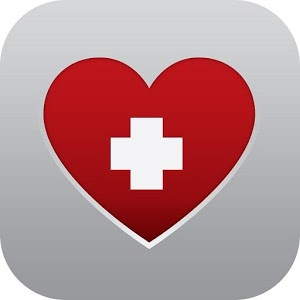
\includegraphics[height=1cm]{PSCV_icon.jpg}

\noindent
Permite calcular una aproximación del riesgo cardicovascular con los fines y tratamientos asociados a cada nivel de riesgo. Ofrece información sobre el diagnóstico, manejo y seguimiento en la diabetes tipo 2, hipertension arterial, infarto agúdo al miocardio...

\noindent
\textbf {ASCVD Risk Estimator}

\noindent

\includegraphics[height=1cm]{ASCVD_icon.jpg}

\noindent
Proporciona acceso rápido a recomendaciones específicas para los riesgos estimados por el calculador a la vez que vez que referncia información relacionado con terápia, monitorización y estilo de vida que puede interesar a pacientes y médicos.

En definitiva, hay varias aplicaciones con una meta temática afín. No obstante, nuestra aplicación presenta funcionalidades únicas no cubiertas por las mencionadas anteriormente que le proporciona un carácter innovador. 

%ESTRUCTURA DE LA MEMORIA
\section{Estructura de la mem\'oria}

La memória está organizada en cinco capitulos siendo el primero de estos la presente introducción.

En el capítulo 2 se hace una explicación detallada de las funcionalidades de la aplicación móvil. Incluyendo los respectivos diagramas de actividades de cada uno de ellos.

El cápitulo 3 presenta los módulos que conforman el sistema.

El cápitulo 4 presenta las tecnologías empleadas acompañadas de una breve descripción y características.

En el cápitulo 5 se presentan las principales conclusiones de este trabajo. En un último lugar se listan las mejoras que se podrían realizar con el fin de incrementar sus funcionalidades y acrecentar su competitividad en el mercado.

%%%%%%%%%%%%%%%%%%%%%%%%%%%%%%%%%%%%%%%%%%%%%%%%%INTRODUCCIÓN EN iNGLÉS%%%%%%%%%%%%%%%%%%%%%%%%%%%%%%%%%%%%%%%%%%%%%%%%%%%%%%%%%%%%%
\addtocounter{chapter}{-1}
\selectlanguage{english}
\chapter{Introduction}

The constant evolution towards a more connected society to get solutions to problems by computerizing the processes and methods and getting closer to the terms of IoT, SmartCities ...

With this idea in mind and after a meeting with the doctor Rafael Rubio Diaz we focus on diabetes as a starting point. They were intended to improve the process of information processing in patients with diabetes to go beyond conventional methods, write medical reports on the computer in their office, to have a mechanism that would allow them not to be tied to their computer and could move around the hospital getting the same end.

Finally, it was decided to expand the project to cardiovascular risk factors to have a more complete and robust application, and to obtain a treatment with more precision, to the doctors to possess more information of the patient.

This project emerges as an Degree Final Work corresponding to the Degree in Computer Engineering, with the firm idea of developing a mobile application that would be able to help within the healthcare framework, giving rapid calculation in the cardiovascular risk of patients.

Surge este proyecto como Trabajo Fin de Grado correspondiente al Grado en Ingeniería Informática, con la firme idea de desarrollar una aplicación movil que fuera capaz de ayudar en el marco de la sanidad, dando rapidez en el cálculo del riesgo cardiovascular de los pacientes.

%MOTIVATION
\section{Motivation}

We wanted to carry out a project that was not only for academic purposes, but was also of no use to a group of society.

We decided to focus on the health sector by several influential factors, as it was a field that we found very interesting and was not as cutting edge as other branches and that there were many applications in the market that covered this specific need.
This application would allow the physician to calculate the cardiovascular risk and store the patient's current medical data, but giving him greater freedom and promptness at the same time as approaching the new technologies.

\vfill
%OBJECTIVES
\section{Objectives}

The overall objective of the project is to develop a tool, a mobile application, that facilitates the work of health personnel in the calculation of cardiovascular risk, storage of patient data and subsequent treatment.

The present Work End of Degree has the following objectives:
\begin{itemize}
	\item Carry out a study of cardiovascular risk factors, to classify them and obtain those that are most relevant for the subsequent calculation of cardiovascular risk.
	\item Design and build a mobile application that is user-friendly, visually appealing and intuitive.
	\item Obtain from all the entered data of a patient, the cardiovascular risk index and an initial treatment.
\end{itemize}

%STATE OF THE ART
\section{State of the art}

In order to determine the degree of impact that this project may have, we have carried out an investigation of possible applications with similar objectives or traits. Our study has revealed the existence of several applications with similar traits, or goals similar to those planned by our application. We cite below several of the potential competitors:

\noindent
\textbf {Appteca }

\noindent

\includegraphics[height=1cm]{riesgo-cardiovascular_icon.jpg}  

\includegraphics[height=1cm]{hipertension_icon.jpg}

\noindent
It is a project carried out by the Spanish Society of Cardiology and the Spanish Society of Medicine, which include several applications related to cardiovascular risk; Cardiovascular risk and Hypertension.

\noindent
\textbf {PSCV}

\noindent
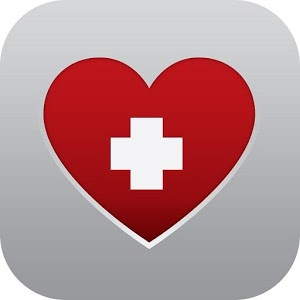
\includegraphics[height=1cm]{PSCV_icon.jpg}

\noindent
It allows to calculate an approximation of the cardiovascular risk with the purposes and treatments associated to each level of risk. It offers information on the diagnosis, management and follow-up in type 2 diabetes, hypertension, myocardial infarction ...

\noindent
\textbf {ASCVD Risk Estimator}

\noindent

\includegraphics[height=1cm]{ASCVD_icon.jpg}

\noindent
It provides quick access to specific recommendations for the calculator's estimated risks, while referring to information related to therapy, monitoring and lifestyle that may be of interest to patients and physicians.

In short, there are several applications with a related thematic goal. However, our application presents unique functionalities not covered by the aforementioned that provides an innovative character. 

%MEMORY STRUCTURE
\section{Memory structure}

The memory is organized in five chapters and the first of these is the present introduction.

Chapter 2 provides a detailed explanation of the features of the mobile application. Including the respective activity diagrams of each of them.

Chapter 3 presents the modules that make up the system.

Chapter 4 presents the technologies used, accompanied by a brief description and characteristics.

In chapter 5 the main conclusions of this work are presented. Finally, we list the improvements that could be made in order to increase its functionality and increase its competitiveness in the market.

%%%%%%%%%%%%%%%%%%%%%%%%%%%%%%%%%%%%%%%%%%%%%%%ESPECIFICACIÓN DE LA APLICACION%%%%%%%%%%%%%%%%%%%%%%%%%%%%%%%%%%%%%%%%%%%%%%%%%%%%%%%%%%
\chapter{Especificación de la aplicaci\'on}

????? ????????????? ????????????? ????????????? ????????????? ?????????????

%%%%%%%%%%%%%%%%%%%%%%%%%%%%%%%%%%%%%%%%%%%%%%%ARQUITECTURA DE LA APLICACIÓN%%%%%%%%%%%%%%%%%%%%%%%%%%%%%%%%%%%%%%%%%%%%%%%%%%%%%%%%%%%
\chapter{Arquitectura de la aplicaci\'on}

????? ????????????? ????????????? ????????????? ????????????? ?????????????

%%%%%%%%%%%%%%%%%%%%%%%%%%%%%%%%%%%%%%%%%%%%%%%%%%%%TECNOLOGIAS%%%%%%%%%%%%%%%%%%%%%%%%%%%%%%%%%%%%%%%%%%%%%%%%%%%%%%%%%%%%%%%
\chapter{Tecnolog\'ias}

????? ????????????? ????????????? ????????????? ????????????? ?????????????

%%%%%%%%%%%%%%%%%%%%%%%%%%%%%%%%%%%%%%%%%%%%%%%%%CONCLUSIONES Y TRABAJO FUTURO%%%%%%%%%%%%%%%%%%%%%%%%%%%%%%%%%%%%%%%%%%%%%%%%%%%%%%%%
\chapter{Conclusiones y trabajo futuro}

????? ????????????? ????????????? ????????????? ????????????? ????????????? 

% BIBLIOGRAFIA                                 
\begin{thebibliography}{10}

%ARTICULO                                                          
\bibitem{light}
   Jennifer~S. Light.
   \newblock When computers were women.
   \newblock \textit{Technology and Culture}, 40:3:455--483, juliol, 1999.

% LIBRO                       
\bibitem{ifrah}
   Georges Ifrah.
   \newblock \textit{Historia universal de las cifras}.
   \newblock Espasa Calpe, S.A., Madrid, sisena edició, 2008.


% URL                                                        
\bibitem{WAR}
   Comunicat de premsa del Departament de la Guerra, 
   emés el 16 de febrer de 1946. 
   \newblock Consultat a 
   \url{http://americanhistory.si.edu/comphist/pr1.pdf}.

\end{thebibliography}
\cleardoublepage


%APENDICES                    
\APPENDIX


% LA CONFIGURACIO DEL SISTEMA                         
\chapter{Manual de instalación}

????? ????????????? ????????????? ????????????? ????????????? ?????????????

\chapter{Manual de usuario}

????? ????????????? ????????????? ????????????? ????????????? ?????????????


\end{document}
